\documentclass[11pt]{beamer}
%\usetheme{Marburg}
\usetheme{Madrid}
\usepackage[utf8]{inputenc}
\usepackage[francais]{babel}
\usepackage[T1]{fontenc}
\usepackage{amsmath}
\usepackage{amsfonts}
\usepackage{amssymb}
\usepackage{graphicx}
\usepackage{tikz}
\title{Approximation numérique de problèmes de convection sur la sphère par un schéma compact}
\setbeamercovered{transparent} 
\setbeamertemplate{navigation symbols}{} 
\author[M. Brachet]{\underline{Matthieu Brachet}, Jean-Pierre Croisille}
\logo{iecl.jpg} 
\date[11.05.2016]{Mercredi 11 Mai 2016}
\institute[IECL]{Institut Elie Cartan de Lorraine (Metz)}
\begin{document}

\begin{frame}
\titlepage
\includegraphics[scale=0.3]{iecl.jpg}
%\includegraphics[scale=0.3]{ul.gif}
\end{frame}

\begin{frame}
\begin{enumerate}
\item Introduction

\item Equation d'advection sphérique

\item Cubed-Sphere et opérateurs aux différences hermitiens sur la sphère
\end{enumerate}
\end{frame}


% *****
\begin{frame}
Résolution d'EDPs sur la sphère :
\begin{block}{Equation de convection :}
\begin{equation*}
\dfrac{\partial h}{\partial t} + \mathbf{a} \left( t, \mathbf{x}\right) \cdot \nabla_T h = 0
\end{equation*}

avec $\mathbf{a} \in \mathbb{T} \mathbb{S}^2$.
\end{block}

\begin{block}{Equation Shallow Water}
\begin{equation*}
\left \{
\begin{array}{r @{=} l}
\partial_t h + \nabla_T \left( \mathbf{u} h \right) & 0\\
\partial_t \left(h \mathbf{u}\right) + \nabla_T \cdot \left( h \mathbf{u} \otimes \mathbf{u} + \dfrac{1}{2} g h^2 \mathbb{I}d \right) & -f \mathbf{k} \wedge \mathbf{u} 
\end{array}
\right.
\end{equation*}
$f$ : force de Coriolis, $g$ : force de gravité et $\mathbf{k}$ la normale extérieure.
\end{block}

\begin{columns}
\column{0.45\textwidth}
\begin{block}{Géométrie sphérique :}
$\nabla_T$, $\nabla_T \cdot $ : opérateurs intrinsèques sur la sphère.
\end{block}

\column{0.45\textwidth}
\begin{block}{Climatologie numérique : }
Simulation sur des temps physiques importants.
\end{block}

\end{columns}


\end{frame}

% *****
\begin{frame}{Cas test de la rotation solide [Williamson, 1992]}
\begin{block}{}
$\bullet$ $(\lambda, \theta)$ : longitude, latitude par rapport à l'axe $(NS)$

$\bullet$ $(\lambda', \theta')$ : longitude, latitude (axe $(NS)$ pivoté de $\alpha$).
\end{block}

\begin{columns}
\column{0.45\textwidth}
\begin{figure}
\def\svgwidth{0.6 \textwidth}
\vspace{0.5cm}
\input{drawing34.pdf_tex}
\end{figure}
\column{0.45\textwidth}
\begin{block}{}
\begin{equation*}
\left \{
\begin{array}{l}
\dfrac{\partial h}{\partial t} + \mathbf{a} \left( \mathbf{x} \right) \cdot \nabla_T h = 0\\[6pt]
h(0,\mathbf{x}) = h_0(\mathbf{x})\\
\end{array}
\right.
\end{equation*}

avec $\mathbf{a} \left( \lambda', \theta' \right) = \omega_0  cos \theta' \mathbf{e}_{\lambda'}$.
\end{block}
\end{columns}

\begin{block}{}
Solution :
$$h \left( \mathbf{x} , t \right) = h_0 \left( R_{\omega_0 t}^{-1} \mathbf{x} \right)$$
avec $R_{\theta}$ matrice de rotation d'angle $\theta$.

\end{block}


\end{frame}



% *****

\begin{frame}{Difficultés numériques}
\begin{columns}
\column{0.3\textwidth}
$\bullet$ Schéma dispersif
\begin{figure}
\href{run:ref_7363895058_test_0.avi}{\includegraphics[scale=0.1]{img_bump.png}} 
\end{figure}

\column{0.3\textwidth}
$\bullet$ Schéma dissipatif
\begin{figure}
\href{run:ref_7363895782_test_0.avi}{\includegraphics[scale=0.1]{img_bump.png}} 
\end{figure}

\column{0.3\textwidth}
$\bullet$ Schéma acceptable
\begin{figure}
\href{run:ref_7363896161_test_0.avi}{\includegraphics[scale=0.1]{img_bump.png}} 
\end{figure}
\end{columns}
\end{frame}

% *****
\begin{frame}{Approximation de $\partial_x u(x_j)$ sur grille cartésienne}
\begin{block}{Approximation d'ordre 2 : $\delta_x u_j$}
\begin{equation*}
\bullet \;\;\; \delta_x u_j = \dfrac{u_{j+1}- u_{j-1}}{2h}
\end{equation*}
\begin{equation*}
\bullet \;\;\; \delta_x u_j = \partial_x u(x_j) + \dfrac{h^2}{6} \partial^{(3)}_x u(x_j) + \mathcal{O}\left( h^4 \right)
\end{equation*}
\end{block}

\begin{block}{Approximation d'ordre 4 : $\bar{\delta}_x u_j$}
\begin{equation*}
\bullet \;\;\; \dfrac{1}{6}\bar{\delta}_x u_j+\dfrac{2}{3}\bar{\delta}_x u_j + \dfrac{1}{6}\bar{\delta}_x u_{j-1} = \dfrac{u_{j+1}- u_{j-1}}{2h}
\end{equation*}

\begin{equation*}
\bullet \;\;\; \bar{\delta}_x u_j = \partial_x u(x_j) - \dfrac{h^4}{180} \partial^{(5)}_x u (x_j) + \mathcal{O}\left( h^6 \right)
\end{equation*}
\end{block}
\end{frame}

% *****

\begin{frame}{Grille sphérique quasi-cartésienne : la grille Cubed-Sphere}
\begin{columns}
\column{0.45\textwidth}
\tiny
\begin{figure}
\def\svgwidth{0.55 \textwidth}
\vspace{0.5cm}
\input{drawing12.pdf_tex}
\end{figure}
\begin{figure}
\begin{center}
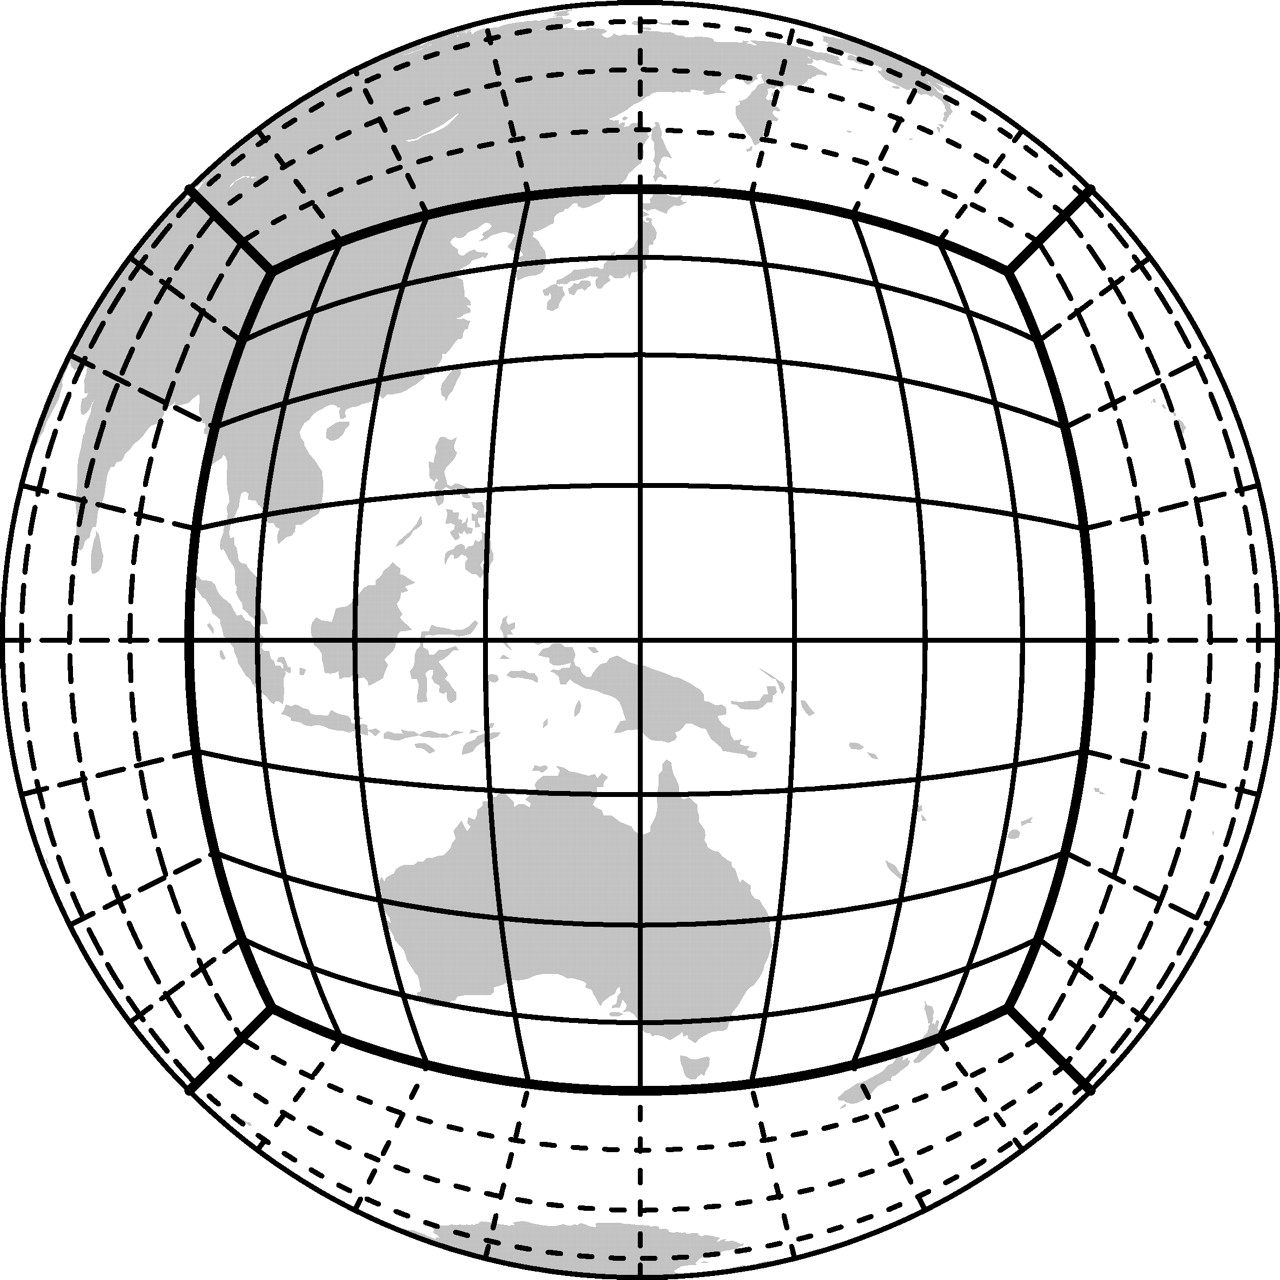
\includegraphics[scale=0.06]{CS_grid.jpg}
\end{center}
\end{figure}

\column{0.45\textwidth}
\begin{itemize}
\item 6 réseaux de cercles géodésiques $C_i^{(1)}$ et $C_j^{(2)}$ , $-N/2 \leq i,j \leq N/2$,

\item $\mathbf{x}_{i,j}=C_i^{(1)} \cap C_i^{(2)}$

\item $C_0^{(1)}$ et $C_0^{(2)}$ se coupent à $90^o$,

\item Grille Cubed-Sphere : 6 panels de $(N+1) \times (N+1)$ points couvrant la sphère.
\end{itemize}
\end{columns}
\end{frame}

\begin{frame}{Métrique sur un panel de la Cubed-Sphere :}
\begin{columns}
\column{0.45\textwidth}
\begin{figure}
\begin{center}
\includegraphics[scale=0.2]{xieta.png}
\end{center}
\caption{1 panel}
\end{figure}

\column{0.45\textwidth}
\begin{block}{}
$\bullet$ Coordonnées locales : angles équatoriaux $- \pi/4 \leq \xi, \eta \leq \pi/4$ ,
\end{block}

\begin{block}{}
\begin{itemize}
\item base locale : $(\mathbf{g}_{\xi}, \mathbf{g}_{\eta} ) = ( \partial_{\xi} \mathbf{x}, \partial_{\eta} \mathbf{x} )$,

\item Tenseur métrique :
$$G = \begin{pmatrix}
\mathbf{g}_{\xi} \cdot \mathbf{g}_{\xi} & \mathbf{g}_{\xi} \cdot \mathbf{g}_{\eta} \\ 
\mathbf{g}_{\eta} \cdot \mathbf{g}_{\xi} & \mathbf{g}_{\eta} \cdot \mathbf{g}_{\eta}
\end{pmatrix} $$

\item base duale :
\begin{equation*}
\left\{
\begin{array}{ccc}
G_{1,1}\mathbf{g}^{\xi} + G_{1,2}\mathbf{g}^{\eta} & = & \mathbf{g}_{\xi} \\ 
G_{2,1}\mathbf{g}^{\xi} + G_{2,2}\mathbf{g}^{\eta} & = & \mathbf{g}_{\eta} \\ 
\end{array} 
\right.
\end{equation*}


\end{itemize}
\end{block}
\end{columns}
\end{frame}



\begin{frame}{Gradient sphérique approché}
\begin{block}{}
Gradient sphérique en $\mathbf{x} ( \xi, \eta)$ :
$$\nabla_T u( \mathbf{x} ) = \dfrac{\partial u}{\partial \xi} ( \mathbf{x} ) _{| \eta} \mathbf{g}^{\xi} (\mathbf{x}) + \dfrac{\partial u}{\partial \eta} ( \mathbf{x} ) _{| \xi} \mathbf{g}^{\eta} (\mathbf{x})$$
\end{block}

\begin{block}{}
Gradient approché en $\mathbf{x}_{i,j}$ :
$$\nabla_{T,h} u_{i,j}  =  u_{\xi,i,j} \mathbf{g}^{\xi} (\mathbf{x}_{i,j}) + u_{\eta, i, j} \mathbf{g}^{\eta} (\mathbf{x}_{i,j})$$
\end{block}

Approximation hermitienne pour $u_{\xi, i, j}$ et $u_{\eta, i, j}$ :

\begin{block}{}
\begin{equation*}
\dfrac{1}{6}u_{\xi,i+1,j}+\dfrac{2}{3}u_{\xi,i,j} + \dfrac{1}{6}u_{\xi,i-1,j} = \dfrac{u_{i+1,j}- u_{i-1,j}}{2\Delta \xi}
\end{equation*}
\begin{equation*}
\dfrac{1}{6}u_{\eta,i,j+1}+\dfrac{2}{3}u_{\eta,i,j} + \dfrac{1}{6}u_{\eta,i,j-1} = \dfrac{u_{i,j+1}- u_{i,j-1}}{2 \Delta \eta}
\end{equation*}
\end{block}
\end{frame}




\begin{frame}{Calcul effectif de $\nabla_{T,h}$}

\begin{block}{}
$\bullet$ Arrangement des données $u_{i,j}$ sur des réseaux de grands cercles,

$\bullet$ Sens intrinsèque du gradient discret $\nabla_{T,h}$.
\end{block}

\begin{columns}
\column{0.45\textwidth}
\begin{figure}
\begin{center}
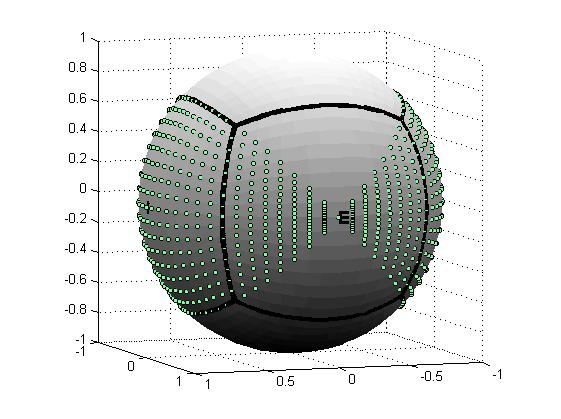
\includegraphics[scale=0.25]{fig22.jpg}
\end{center}
\end{figure}
\column{0.45\textwidth}
\begin{figure}
\begin{center}
\includegraphics[scale=0.2]{fig72.jpg}
\end{center}
\end{figure}
\end{columns}


\end{frame}

\begin{frame}{Consistance de $\nabla_{T,h}$}

\begin{block}{Proposition}
Soit $u : \mathbb{S}^2 \rightarrow \mathbb{R}$ régulière alors :
\begin{equation*}
\| \nabla_{T,h} u_{i,j} - \nabla_T u (\mathbf{x}_{i,j}) \| = \mathcal{O} \left( \Delta \xi^3, \Delta \eta^3 \right)
\end{equation*}
\end{block}

\textbf{Remarque :} en pratique, ordre 4 observé.

\end{frame}






\begin{frame}{Equation de convection avec vitesse dépendant du temps}

\begin{block}{}
\begin{equation}
\left \{
\begin{array}{l}
\dfrac{\partial h}{\partial t} + \mathbf{a}(t,\mathbf{x}) \cdot \nabla_T h = 0\\[6pt]
h(0,\mathbf{x}) = h_0(\mathbf{x})\\
\end{array}
\right.
\label{eq:advection}
\end{equation}
\end{block}

\begin{block}{vitesse de type vortex indépendant du temps}
$\mathbf{a}_r(\mathbf{x}) = \omega_r (\theta') cos ( \theta') \mathbf{e}_{\lambda'}$ vitesse variable du vortex.
\end{block}


\begin{block}{Vitesse globale :
Combinaison de la rotation solide et de la vitesse de type vortex}

$$\mathbf{a}(t, \mathbf{x}) = \underbrace{\mathbf{a}_s ( \mathbf{x} )}_{\text{rotation solide}} + \underbrace{\mathbf{a}_r (t, \mathbf{x})}_{\text{vitesse de type vortex}}$$




\begin{flushright}
[Nair, Jablonowski, 2008]
\end{flushright}
\end{block}

\end{frame}



\begin{frame}
\begin{block}{Solution analytique}
Solution analytique de \eqref{eq:advection} donnée dans $( \lambda', \theta')$, le système de coordonnées associé à l'axe tourné d'un angle $\alpha$, par :

$$h(t, \lambda', \theta') = 1 -tanh \left[ \frac{\rho}{\gamma} sin( \lambda' - \omega_r t ) \right]$$

$\rho$ et $\omega_r$ dépendant de $\theta'$.
\end{block}

\begin{columns}
\column{0.45\textwidth}
\begin{figure}
\href{run:ref_7363145849_test_2.avi}{\includegraphics[scale=0.25]{14-Oct-2015_normerreur_test_2.png}} 
\caption{maillage $6 \times 40 \times 40$}
\end{figure}

\column{0.45\textwidth}
Discrétisation en temps RK4 + Filtrage à l'ordre 10
\end{columns}

\end{frame}


\begin{frame}{Table de convergence pour le test du vortex en déplacement}
\begin{table}
\begin{tabular}{c||cc|cc|cc}
$N$ & $max_n |e_1^n|$ & ordre  & $max_n |e_2^n|$ & ordre  & $max_n |e_{\infty}^n|$ & ordre \\
\hline
\hline
$40$ & $2.7609 (-3)$ & -  & $9.7386 (-3)$ & - & $5.4808 (-2)$  & - \\
\hline 
$50$ & $1.2760 (-3)$ & $3.5364$ & $5.0160 (-3)$ & $3.0399$ & $3.2035 (-2)$ & $2.4605$ \\
\hline
$60$ & $6.2957 (-4)$ & $3.9456$ & $2.6157 (-3)$ & $3.6365$ & $1.8218 (-2)$ & $3.1523$ \\
\hline
$80$ & $1.9603 (-4) $ & $4.1145$ & $8.3722 (-4)$ & $4.0173$ & $6.0931 (-3)$ & $3.8623$ \\
\hline
$100$ & $8.0399 (-5)$ & $4.0389$ & $3.4524 (-4)$ & $4.0143$ & $2.6514 (-3)$ & $3.7706$\\
\hline
$150$ & $1.5656 (-5)$ & $4.0684$ & $6.9199 (-5)$ & $3.9966$ & $5.8082 (-4)$ & $3.7756$
\end{tabular}
\caption{Table de convergence pour le test du vortex en déplacement, $CFL = 0.7$ ; $\alpha = \pi /4$.}\end{table}

\end{frame}





\begin{frame}{Objectif : équation de Saint-Venant linéarisé avec force de Coriolis (LSWEC)}

\begin{block}{LSWEC}
$\mathbf{u}( t, \mathbf{x}) $, $h( t, \mathbf{x})$ : perturbations de vitesse et de hauteur.

\begin{equation}
\left \{
\begin{array}{l}
\partial_t \mathbf{u}+g \nabla_T h  = - f \mathbf{k} \wedge \mathbf{u}\\
\partial_t h + H_0 \nabla_T \cdot \mathbf{u} = 0\\
h(0, \mathbf{x} ) = h_0 ( \mathbf{x} )\\
\mathbf{u}(0, \mathbf{x} ) = \mathbf{u}_0 ( \mathbf{x} )\\
\end{array}
\right.
\label{eq:LSWEC}
\end{equation}
\end{block}

\begin{block}{Divergence :}
Si $\mathbf{F} : \mathbb{S}^2 \rightarrow \mathbb{T}\mathbb{S}^2$ alors la divergence en $\mathbf{x}(\xi, \eta)$ est :

\begin{equation*}
\nabla_T \cdot  \mathbf{F} ( \mathbf{x}_{i,j} ) = \dfrac{1}{\sqrt{\overline{G}}} \left[ \dfrac{\partial}{\partial \xi} \left( \sqrt{\overline{G}} \mathbf{F} \cdot \mathbf{g}^{\xi}   \right)_{| \eta} + \dfrac{\partial}{\partial \eta} \left( \sqrt{\overline{G}} \mathbf{F} \cdot \mathbf{g}^{\eta}   \right)_{| \xi}\right]
\end{equation*}
\end{block}

avec $\overline{G} = | det \left( G \right) |$.
\end{frame}



\begin{frame}
\begin{block}{Divergence sphérique approchée :}
La divergence approchée en $\mathbf{x}_{i,j}$ est :
\begin{equation*}
\nabla_{T,h} \cdot \mathbf{F}_{i,j} = \dfrac{1}{\sqrt{\overline{G}}} \left[  \left( \sqrt{\overline{G}} \mathbf{F} \cdot \mathbf{g}^{\xi}   \right)_{\xi, i, j} +  \left( \sqrt{\overline{G}} \mathbf{F} \cdot \mathbf{g}^{\eta}   \right)_{\eta, i, j}\right]
\end{equation*}
\end{block}

\begin{block}{Observation numérique}
$$\| \nabla_T \cdot \mathbf{F} ( \mathbf{x}_{i,j} )  - \nabla_{T,h} \cdot \mathbf{F}_{i,j}  \| = \mathcal{O} \left( \Delta \xi^4, \Delta \eta^4 \right)$$
\end{block}

\end{frame}

\begin{frame}{Table de convergence pour la divergence}
\begin{block}{Test numérique }
Fonction vectorielle tangentielle de la forme :
\begin{equation}
\nonumber
\mathbf{F}=c(\mathbf{x})( \mathbf{n}(\mathbf{x})\times \mathbf{\phi}),\;\; \nabla_T \cdot \mathbf{F}= \nabla_T c(\mathbf{x})\cdot (\mathbf{n}(\mathbf{x}) \times \mathbf{\phi})
\end{equation}
\tiny
\begin{table}[h!]
\begin{center}
\begin{tabular}{|c|c|c|c|c|c|c|c|}
\hline 
& N=32 & taux & N=64 & taux & N=128 & taux & N=256\\
\hline
\hline 
$e_\infty$ & 1.5372(0) & 4.29 & 7.8539(-2) & 4.07 & 4.6704(-3) & 4.02& 2.8817(-4)\\
\hline 
$\Delta \xi$ en km & 312.5 &  & 156.25 &  & 78.12 &  & 39.06 \\
\hline
Nb de points de grille & 6146& &  24578 &  & 93306 & & 393218
\\
\hline
\end{tabular}
\vspace{0.2cm}
\caption{\footnotesize Erreur calculée entre la divergence sphérique approchée de
$\mathbf{F}(\mathbf{n})= c(\mathbf{x}) (\mathbf{n}(x) \times \varphi)$ et 
$c(\mathbf{x})=\sin(2 \pi x)+\sin(6 \pi y)+\sin(10 \pi z)$, $\mathbf{\phi}=[1, 1, 1]^T$.
La divergence exacte est $\nabla_T \cdot (\mathbf{F}(\mathbf{x}))= \nabla_T c(\mathbf{x}) . (\mathbf{n}(\mathbf{x}) \times \mathbf{\phi})$. 

}
\label{table:4}
\end{center}
\end{table}

\end{block}
\end{frame}

\begin{frame}
\begin{center}
Merci de votre attention.
\end{center}
\end{frame}




\end{document}
